\documentclass[11pt,a4paper]{article}
\usepackage[utf8]{inputenc}
\usepackage{amsmath}
\usepackage{mathtools}
\usepackage{amsfonts}
\usepackage{amssymb}
\usepackage{graphicx}
\usepackage{caption}
\usepackage{subcaption}
\usepackage{comment}
\usepackage{color}
\usepackage{enumitem}
\usepackage[left=2cm,right=2cm,top=2cm,bottom=2cm]{geometry}
\usepackage{listings}
\usepackage{color}

\setlength{\jot}{10pt}
 
\definecolor{codegreen}{rgb}{0,0.6,0}
\definecolor{codegray}{rgb}{0.5,0.5,0.5}
\definecolor{codepurple}{rgb}{0.58,0,0.82}
\definecolor{backcolour}{rgb}{0.95,0.95,0.92}
 
\lstdefinestyle{mystyle}{
    backgroundcolor=\color{backcolour},   
    commentstyle=\color{codegreen},
    keywordstyle=\color{magenta},
    numberstyle=\tiny\color{codegray},
    stringstyle=\color{codepurple},
    basicstyle=\footnotesize,
    breakatwhitespace=false,         
    breaklines=true,                 
    captionpos=b,                    
    keepspaces=true,                 
    numbers=left,                    
    numbersep=5pt,                  
    showspaces=false,                
    showstringspaces=false,
    showtabs=false,                  
    tabsize=2
}
 
\lstset{style=mystyle}
\graphicspath{ {./figures/} }
\author{Andrew Teta}
\title{ECEN 4532 - Lab 6: Machine Learning}
\date{May 1, 2019}

\begin{document}

\maketitle

\begin{figure}[ht]
	\centering
	
\includegraphics[width=\textwidth]{ml}
\end{figure}

\pagebreak

\tableofcontents

\pagebreak

\section{Introduction}
Researchers in many different fields often collect large quantities of data, with the hope of finding it useful to develop predictions of various phenomena. One very common example in today's age would be advertisement targeting. As users browse the web, certain details about the demographic of people viewing and purchasing products can be collected and stored as a large data set. Machine learning may be a good way to predict what a random user will purchase based on their purchase history or demographic relationship. Many other problems similar to this can be solved using tools like machine learning. Often, they are problems of classification. By classifying users based on their gender, age, region of residency, or other factors, a program or algorithm can predict an outcome for a given activity. The classification involved may be binary or higher order, where a statistic could fall into one of many classification "bins". Other problems may involve continuous predictions. 

When discussing the concept of machine learning, it is helpful to have some motivation and notation. Considering the first example of this lab, we have a domain of objects (passengers on the Titanic) which we would like to classify into categories ("survived or "perished"). Often, the objects are too complex to classify directly and so instead, an array of characteristics for each object are defined as \textit{features}. These features are grouped into a \textit{feature vector}. Each feature vector is referred to as an \textit{instance} and the set of all feature vectors, the \textit{instance space}. 

We will then take a "training set" of data, which correctly maps the instances to its classification. The training set is incomplete and only contains a sample of all the possible instances, so doing our best, we can "learn" an approximation to the real function mapping features to classifications. 

In this lab, we will investigate binary classification using Support Vector Machines, linear regression for predicting a continuous quantity, and multi-class classification using neural networks. The approach here is in the context of data analysis.

\section{Background}
Three data sets will be used for three different classification techniques, respectively. Specifically, we consider:

\begin{itemize}
\item Support Vector Machine (SVM) to predict who survived the sinking of the Titanic. This is an example of a binary classification problem (i.e. "survived" or "perished").
\item Linear regression to predict the water resistance of a sailing yacht based on a selection of design parameters. The predicted value will be a real number here, so this is an example of a continuous classification problem.
\item Neural networking to recognize hand-written digits. This is a multi-class classification problem as there are 10 classes or "bins".
\end{itemize}

For all cases, we will utilize a set of labeled outcomes. As an example, for hand-written digit recognition, we have 70,000 images of numerals 0 through 9, correctly labeled. Thus, we are practicing "supervised" machine learning by fitting an appropriate function to a data set based on a large number of input/output pairs.

\subsection{Support Vector Machines}
A Support Vector Machine (SVM) is a method of binary classification through supervised learning. A model is built based on a training set which can assign a new data point to one classification or the other. It is easiest to understand the process and goal of fitting this model with a graphical representation. Figure \ref{fig:svm} shows that an SVM aims to find the optimal "line", called a \textit{hyperplane} between data points falling into either classification. 

\begin{figure}[ht]
\centering
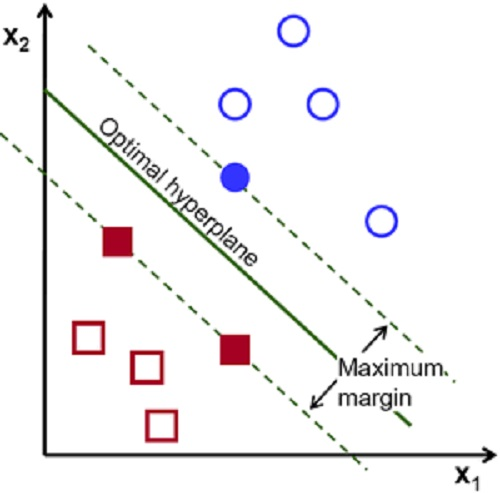
\includegraphics[width=0.4\textwidth]{svm}
\caption{Graphical representation of an SVM hyperplane. \\Credit: https://www.aitrends.com/ai-insider/support-vector-machines-svm-ai-self-driving-cars/}
\label{fig:svm}
\end{figure}

Calling the hyperplane a "line" is inaccurate because really it forms a plane of separation between the feature vectors, represented by red squares and blue circles in fig. \ref{fig:svm}. This plane lives in multidimensional space. If each support vector has dimension $p$, then the hyperplane is of dimension $p-1$. 

As the graphic suggests, another characteristic of SVMs is the margin of the hyperplane. An optimal hyperplane will maximize the margin, effectively finding the largest separation between classifications. Thus, a new data point will fall more decisively on one side of the hyperplane. Furthermore, the vectors defining the margin are called support vectors.

\subsection{Linear Regression}
Fundamentally, the problem of linear regression seeks to find a "best fit" line passing through a data set, to find a model to which predicted data can be fit. The concept of multiple linear regression deals with more than one independent variable. Linear regression is useful when a data set is "over-determined"--often occurring in scientific or statistical measurement. This would be the case where a solution is desired for only one or two dependent variables, but hundreds or thousands of independent variable samples are collected. Then, rather than a single solution to what has become a linear algebra problem, we now have multiple solutions. Through the following proof, we can show that the "best" solution can be found.
We begin with the assumption that we have a set of $N$ measurements, $x_i$, collected together into a vector,

\begin{align*}
\vec{x} = (x_1, x_2, \ldots, x_N)
\end{align*}

Recall, the length of $\vec{x}^2$ is its "energy". Additionally, we will refer to a vector of constants, all equal to $\mu$ as $\vec{\mu}$.
Then, we can define the average energy per vector component of $\vec{x}$ as the error power and call this the \textit{variance}

\begin{align*}
\sigma^2 = \frac{1}{N} |\vec{x} = \vec{\mu}|^2
\end{align*}

where the vertical bars imply vector length and $\vec{\mu}$ is the mean vector of $\vec{x}$.
Finding \textit{standard deviation}, $\sigma$, we have:

\begin{align*}
\sigma = \frac{1}{\sqrt{N}} |\vec{x} - \vec{\mu}|
\end{align*}

Now, considering the case of data point vectors, $\vec{x}$ and $\vec{y}$ (independent/independent variable pairs) we can begin to find a linear regression.
First, we remap each vector into unit vector form:

\begin{align*}
\vec{w} &= \frac{1}{\sigma_x}(\vec{x} - \vec{\mu_x}) \\
\vec{z} &= \frac{1}{\sigma_y}(\vec{y} - \vec{\mu_y})
\end{align*}

We now seek a line, defined by the scalar constants $a$ and $b$, which minimizes the cost (or error power) and write:

\begin{align*}
C(a,b) = |\vec{z} - (a\vec{w} + \vec{b})|^2
\end{align*}

which can be written as a dot product:

\begin{align*}
C(a,b) &= (\vec{z} = (a\vec{w} + \vec{b})) \cdot (\vec{z} - (a\vec{w} + \vec{b})) \\
&= N - 2a\vec{w} \cdot \vec{z} + a^2 N + Nb^2.
\end{align*}

Then, it is possible to show that $N - 2a\vec{w} \cdot \vec{z} + a^2 N$ is a parabola in terms of $a$ and has its minimum at

\begin{align*}
a &= \frac{\vec{w}\vec{z}}{N} \\
&= \frac{\vec{w}}{\sqrt{N}} \cdot \frac{\vec{z}}{\sqrt{N}} \\
&= cos\theta
\end{align*}

Thus, the value $a$ is the correlation coefficient and is the cosine of the angle between the vectors $\vec{w}$ and $\vec{z}$. For notation consistency with other documentation, we will redefine $a= \rho$ and substitute to arrive at:

\begin{align*}
y = \beta x + (\mu_x - \beta \mu_x), \quad	&\text{where $\beta = \rho \frac{\sigma_y}{\sigma_x}$}
\end{align*}

\subsection{Neural Networks}
The basic building blocks of a neural network are "perceptrons" (fig. \ref{fig:nn}) which compute the dot product of its input vector $\vec{x}$, with its weights, $\vec{w}$. The result is passed through a threshold with respect to a bias, $b$ (fig. \ref{fig:nn1}).

\begin{figure}[ht]
\centering
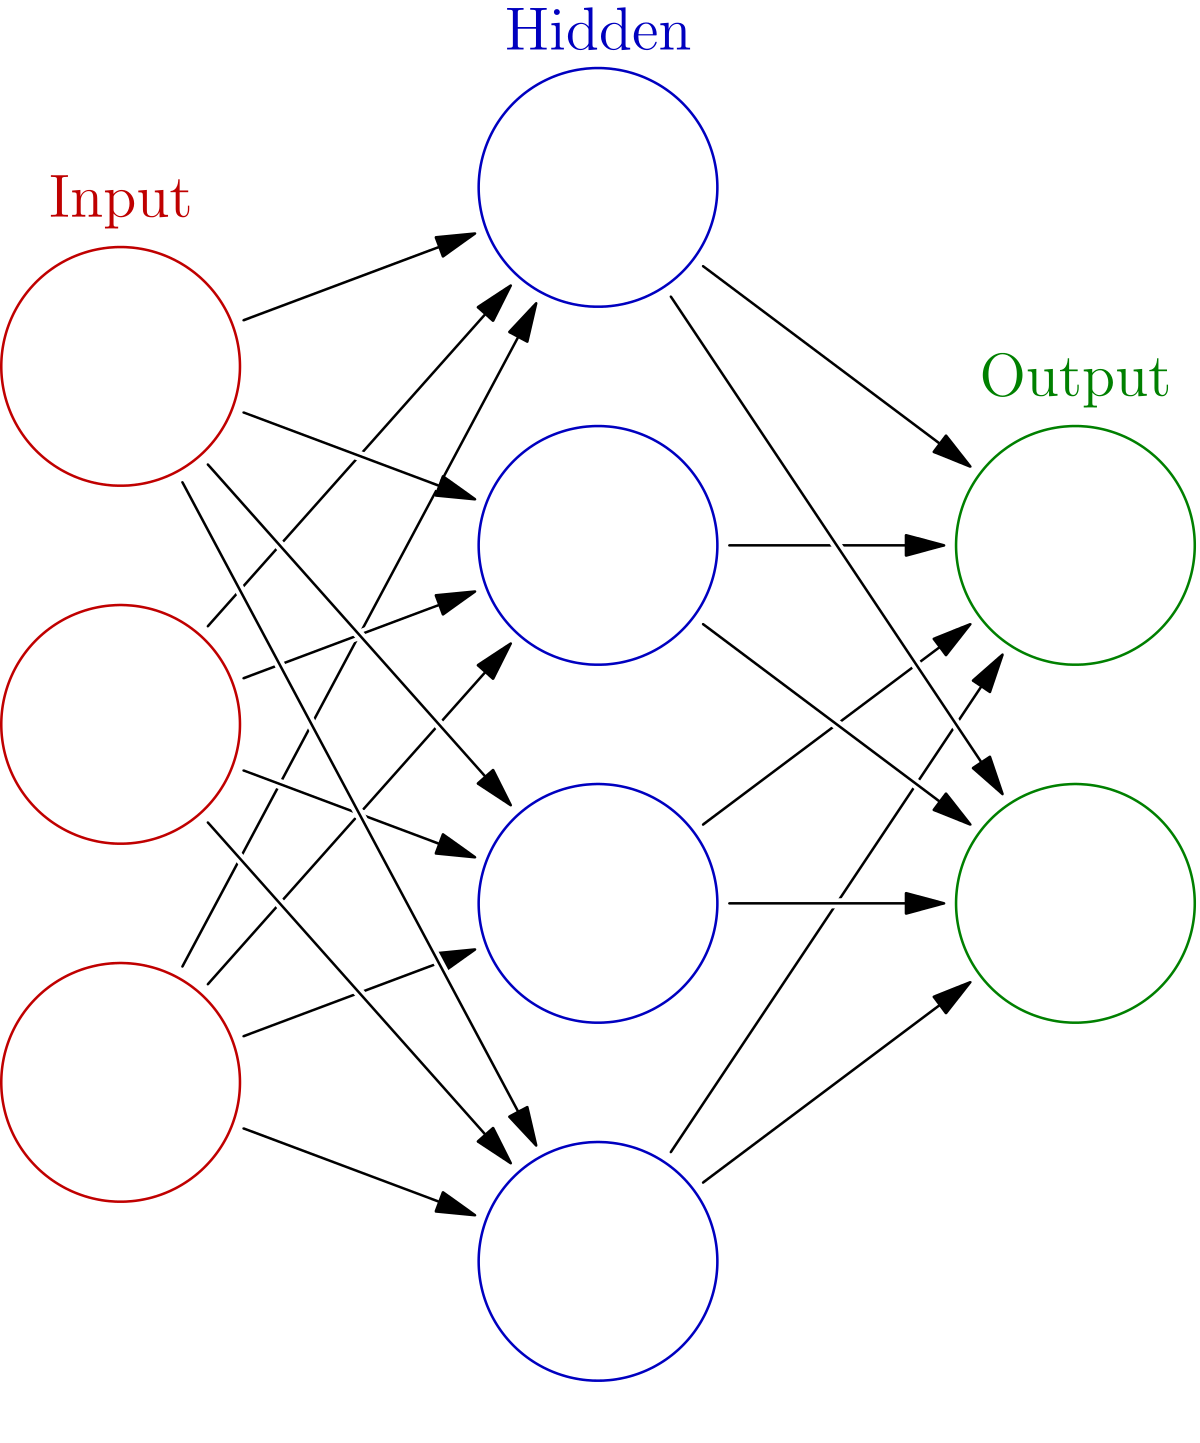
\includegraphics[width=0.4\textwidth]{nn}
\caption{Perceptrons shown on the left.}
\label{fig:nn}
\end{figure}

\begin{figure}[ht]
\centering
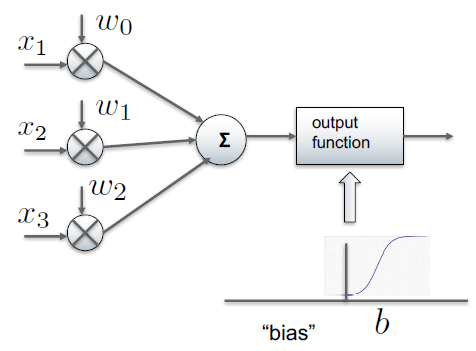
\includegraphics[width=0.6\textwidth]{nn1}
\caption{Inside of a perceptron.}
\label{fig:nn1}
\end{figure}

The process of training a neural network optimizes the parameters of the perceptrons in the network. The hidden layers shown in figure \ref{fig:nn} can be many layers deep and define the complexity of the network, but eventually narrow the input into a single classification at the output layer.

\section{Procedure}
The procedure for this lab is divided into three parts.

\begin{enumerate}
\item Binary classification using an SVM
\item Continuous classification using linear regression
\item Multiple classification using a neural network
\end{enumerate}

\subsection{SVM}
For this portion of the lab, we will be using a training set of data, organized in multiple column fields of a \verb|.csv| file saved to the disk. 

The data set we will be using is a collection of information about passengers who were on the Titanic when it sank. The binary classification we wish to predict is whether each passenger "survived" or "perished". For each passenger, the file contains the following columns:

\begin{itemize}
\item Class
\item Survived
\item Name
\item Sex
\item Age
\item Siblings and Parents
\item Parents and Children
\item Ticket number
\item Fare
\item Cabin
\item Location Embarked
\item Boat
\item Body Weight
\item Destination
\end{itemize}

Utilizing the Python module, \verb|csv|, we can import this table and convert the fields into a \verb|numpy| matrix of support vectors and a vector of labels. Some entries of this \verb|.csv| table are in text format, others in integer, however all entries are initially imported as character arrays and so must be parsed correctly to prepare the data for processing in an SVM. Thus the data import procedure is:

\begin{enumerate}
\item Create \verb|csv| reader object.
\item Iterate through \verb|.csv| file, element by element.
\item Parse individual data fields and build support vectors for each instance
\item Build support vector matrix and label vector
\end{enumerate}

We will not import all columns into our data matrix, but instead use only:

\begin{itemize}
\item Class
\item Sex
\item Age
\item Siblings and Parents
\item Parents and Children
\item Fare
\item Location Embarked
\end{itemize}

and use the "survived" column as our label vector.

Next, we want to analyze this data using the techniques of an SVM. Rather than writing the complex algorithms from scratch, we will utilize a Python module, \verb|SVM| from the package \verb|sklearn|. Then, we feed our support vector matrix and label vector to the \verb|fit()| function to "train" our SVM. Finally, we can run some predictions using the \verb|predict()| function and analyze the performance of our machine. Again, listing the procedure:

\begin{enumerate}
\item Declare a \verb|sklearn| SVM object.
\item \verb|fit()| the SVM to our data set, passing the label vector in.
\item \verb|predict()| an outcome for each instance and measure performance.
\end{enumerate}

\subsubsection{Results}
We started by training the SVM on all features. While the outcome was not bad, the process took a very long time, so we considered limiting the training data set to only three features. Defining the percentage of correctly predicted outcomes as $p$, we found:

\begin{align*}
p = 80.51\%
\end{align*}

To find the optimal features to use, while still achieving similar prediction performance, we ran the SVM training and prediction process on each feature individually. The results for each feature are shown below.

\begin{center}
 \begin{tabular}{||c | c||} 
 \hline
 Feature & Outcome Success (\%) \\ [0.5ex] 
 \hline\hline
 Fare & 66.00 \\ 
 \hline
 Class & 67.68 \\
 \hline
 Sex & 77.99 \\
 \hline
 Age & 66.08 \\
 \hline
 Siblings and Parents & 62.33 \\
 \hline
 Parents and Children & 64.32 \\
 \hline
 Location Embarked & 64.17 \\ [1ex] 
 \hline
\end{tabular}
\end{center}

Having obtained some insight into which features are most correlated with the outcome, we recombined multiple features into our training set. Selecting the three features with best prediction accuracy, we found highest overall accuracy based on age, sex, and class to be:

\begin{align*}
p = 78.99\%
\end{align*}\

which is very close to the performance we had with all features considered. This is a much better solution, because the processing time was much less.

\subsection{Linear Regression}
Again, using \verb|sklearn|, this time we will use a module from the \verb|linear_model| package, called \verb|LinearRegression|. And, you guessed it, this module will help us perform linear regression. 

Overall, the procedure is very similar to what we did for the SVM.

\begin{itemize}
\item Import training data from a \verb|.csv|
	\begin{itemize}
		\item Organize independent variables in a matrix and labels into a vector
	\end{itemize}
\item \verb|fit()| a model to the data, using the label vector
\item \verb|predict| the outcome based on the input
\item Statistically measure the performance
\end{itemize}

For this portion of the lab, we will be using linear regression to fit a model to a set of data containing a list of parameters used in the design of a yacht hull. These design parameters are suspected to contribute to the resulting resistance seen by the yacht against the water. The purpose of this model will then be to accurately measure which parameters contribute most heavily to yacht resistance and fit a model which could then be used to optimize a design.

The design parameters considered are:

\begin{itemize}
\item Longitudinal Position Center of Buoyancy
\item Prismatic Coefficient
\item Length-Displacement Ratio
\item Beam-Draught Ratio
\item Length-Beam Ratio
\item Froude Number
\end{itemize}

And, more formally, the value we wish to predict is the "Residuary resistance per unit weight of displacement."

\subsubsection{Measuring Performance}
It will be important to compare the performance of two regression model predictors and so we will define the two terms,

\begin{itemize}
\item Total Sum of Squares (TSS)
\item Residual Sum of Squares (RSS)
\end{itemize}

Where,

\begin{align*}
TSS = \sum_{i=1}^M (y_i - \mu_y)^2
\end{align*}

and

\begin{align*}
RSS = \sum_{i=1}^M (y_i - \hat{y}_i)^2.
\end{align*}

Then, the "Fraction of Variance Unexplained" is defined as

\begin{align*}
FVU = \frac{RSS}{TSS}
\end{align*}

and the "Coefficient of Determination", $R^2$ as

\begin{align*}
R^2 = 1 - FVU = 1 - \frac{RSS}{TSS}.
\end{align*}

The value $R^2$ is essentially the fraction of variance of $y$ (the outcome) that is "explained" by the prediction. As follows, the quantity, $1-R^2$ is the fraction of variance that is "unexplained" by the prediction. Thus, we should attempt to maximize the value of $R^2$ to find the best prediction model.

\subsubsection{Results}
To begin, we \verb|fit()| a linear regression model to all six design parameters over a range of over 300 sample data points for each. Running the prediction over the training set, we found the value of $R^2 = 0.6575$. Figure \ref{fig:yacht} shows graphically what this outcome looks like. This $R^2$ value is not great, but there are a couple things to consider. First, not all the design parameters are guaranteed to have a significant effect on the outcome, and so could be introducing unnecessary model parameters. Secondly, and also more importantly, we have just trained this regression model with the assumption of a linear relationship between each of the design parameters and outcome.

\begin{figure}[ht]
\centering
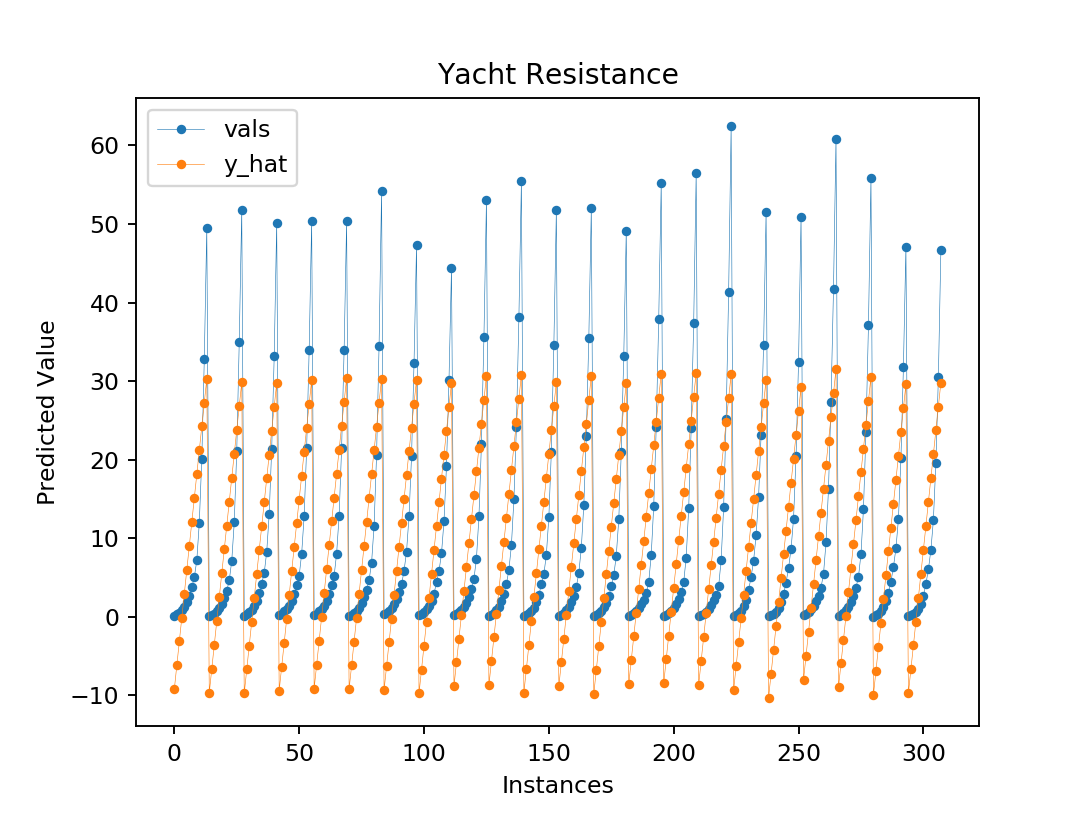
\includegraphics[width=0.6\textwidth]{yacht}
\caption{Comparison of labeled outcomes and predicted outcomes based on a linear regression learning method.}
\label{fig:yacht}
\end{figure}

Considering first, that some parameters may not be contributing much, we ran the same procedure of fitting, predicting, and calculating $R^2$ for each parameter set alone. The results are shown in table \ref{table:yacht}.

\begin{center}\label{table:yacht}
 \begin{tabular}{||c | c||} 
 \hline
 Design Parameter & $R^2$ \\ [0.5ex] 
 \hline\hline
 Longitudinal Position Center of Buoyancy & $0.000372$ \\ 
 \hline
 Prismatic Coefficient & $0.000816$ \\
 \hline
 Length-Displacement Ratio & $8.8e^{-6}$ \\
 \hline
 Beam-Draught Ratio & $0.000154$ \\
 \hline
 Length-Beam Ratio & $1.05e^{-6}$ \\
 \hline
 Froude Number & $0.656$ \\ [1ex] 
 \hline
\end{tabular}
\end{center}

It is easy to see that most parameters do not contribute much to the variance of the outcome, with the highest contenders being:

\begin{enumerate}
\item Froude Number
\item Prismatic Coefficient
\item Longitudinal Position Center of Buoyancy
\end{enumerate}

Taking this into consideration, we ran the procedure again, using only these three parameters. As may have been expected, however, we found $R^2 = 0.6574$, with the remaining significant figures attributed to the other parameters. Since this obviously did not improve our prediction results, we need to look for another cause.

Plotting individually...

\end{document}